\documentclass[../delivery_hospital_report.tex]{subfiles}
\graphicspath{ {images/}{../images/}{../../images/} }
\begin{document}
%================================ CONTROLE ========================
\section{Controle}
####
texto explicando o modulo
    - função principal
    - problema que ela resolve
####

\subsection{Placa}
####
texto explicando a placa
    - areas principais
####

%================================ CONTROLE PROTOTIPO ========================
\subsubsection{Protótipo}

\paragraph{Esquemático}

\begin{figure}[h]
\centering
    \caption{Protótipo placa de Controle - Esquemático principal }
    \centering % para centralizarmos a figura
    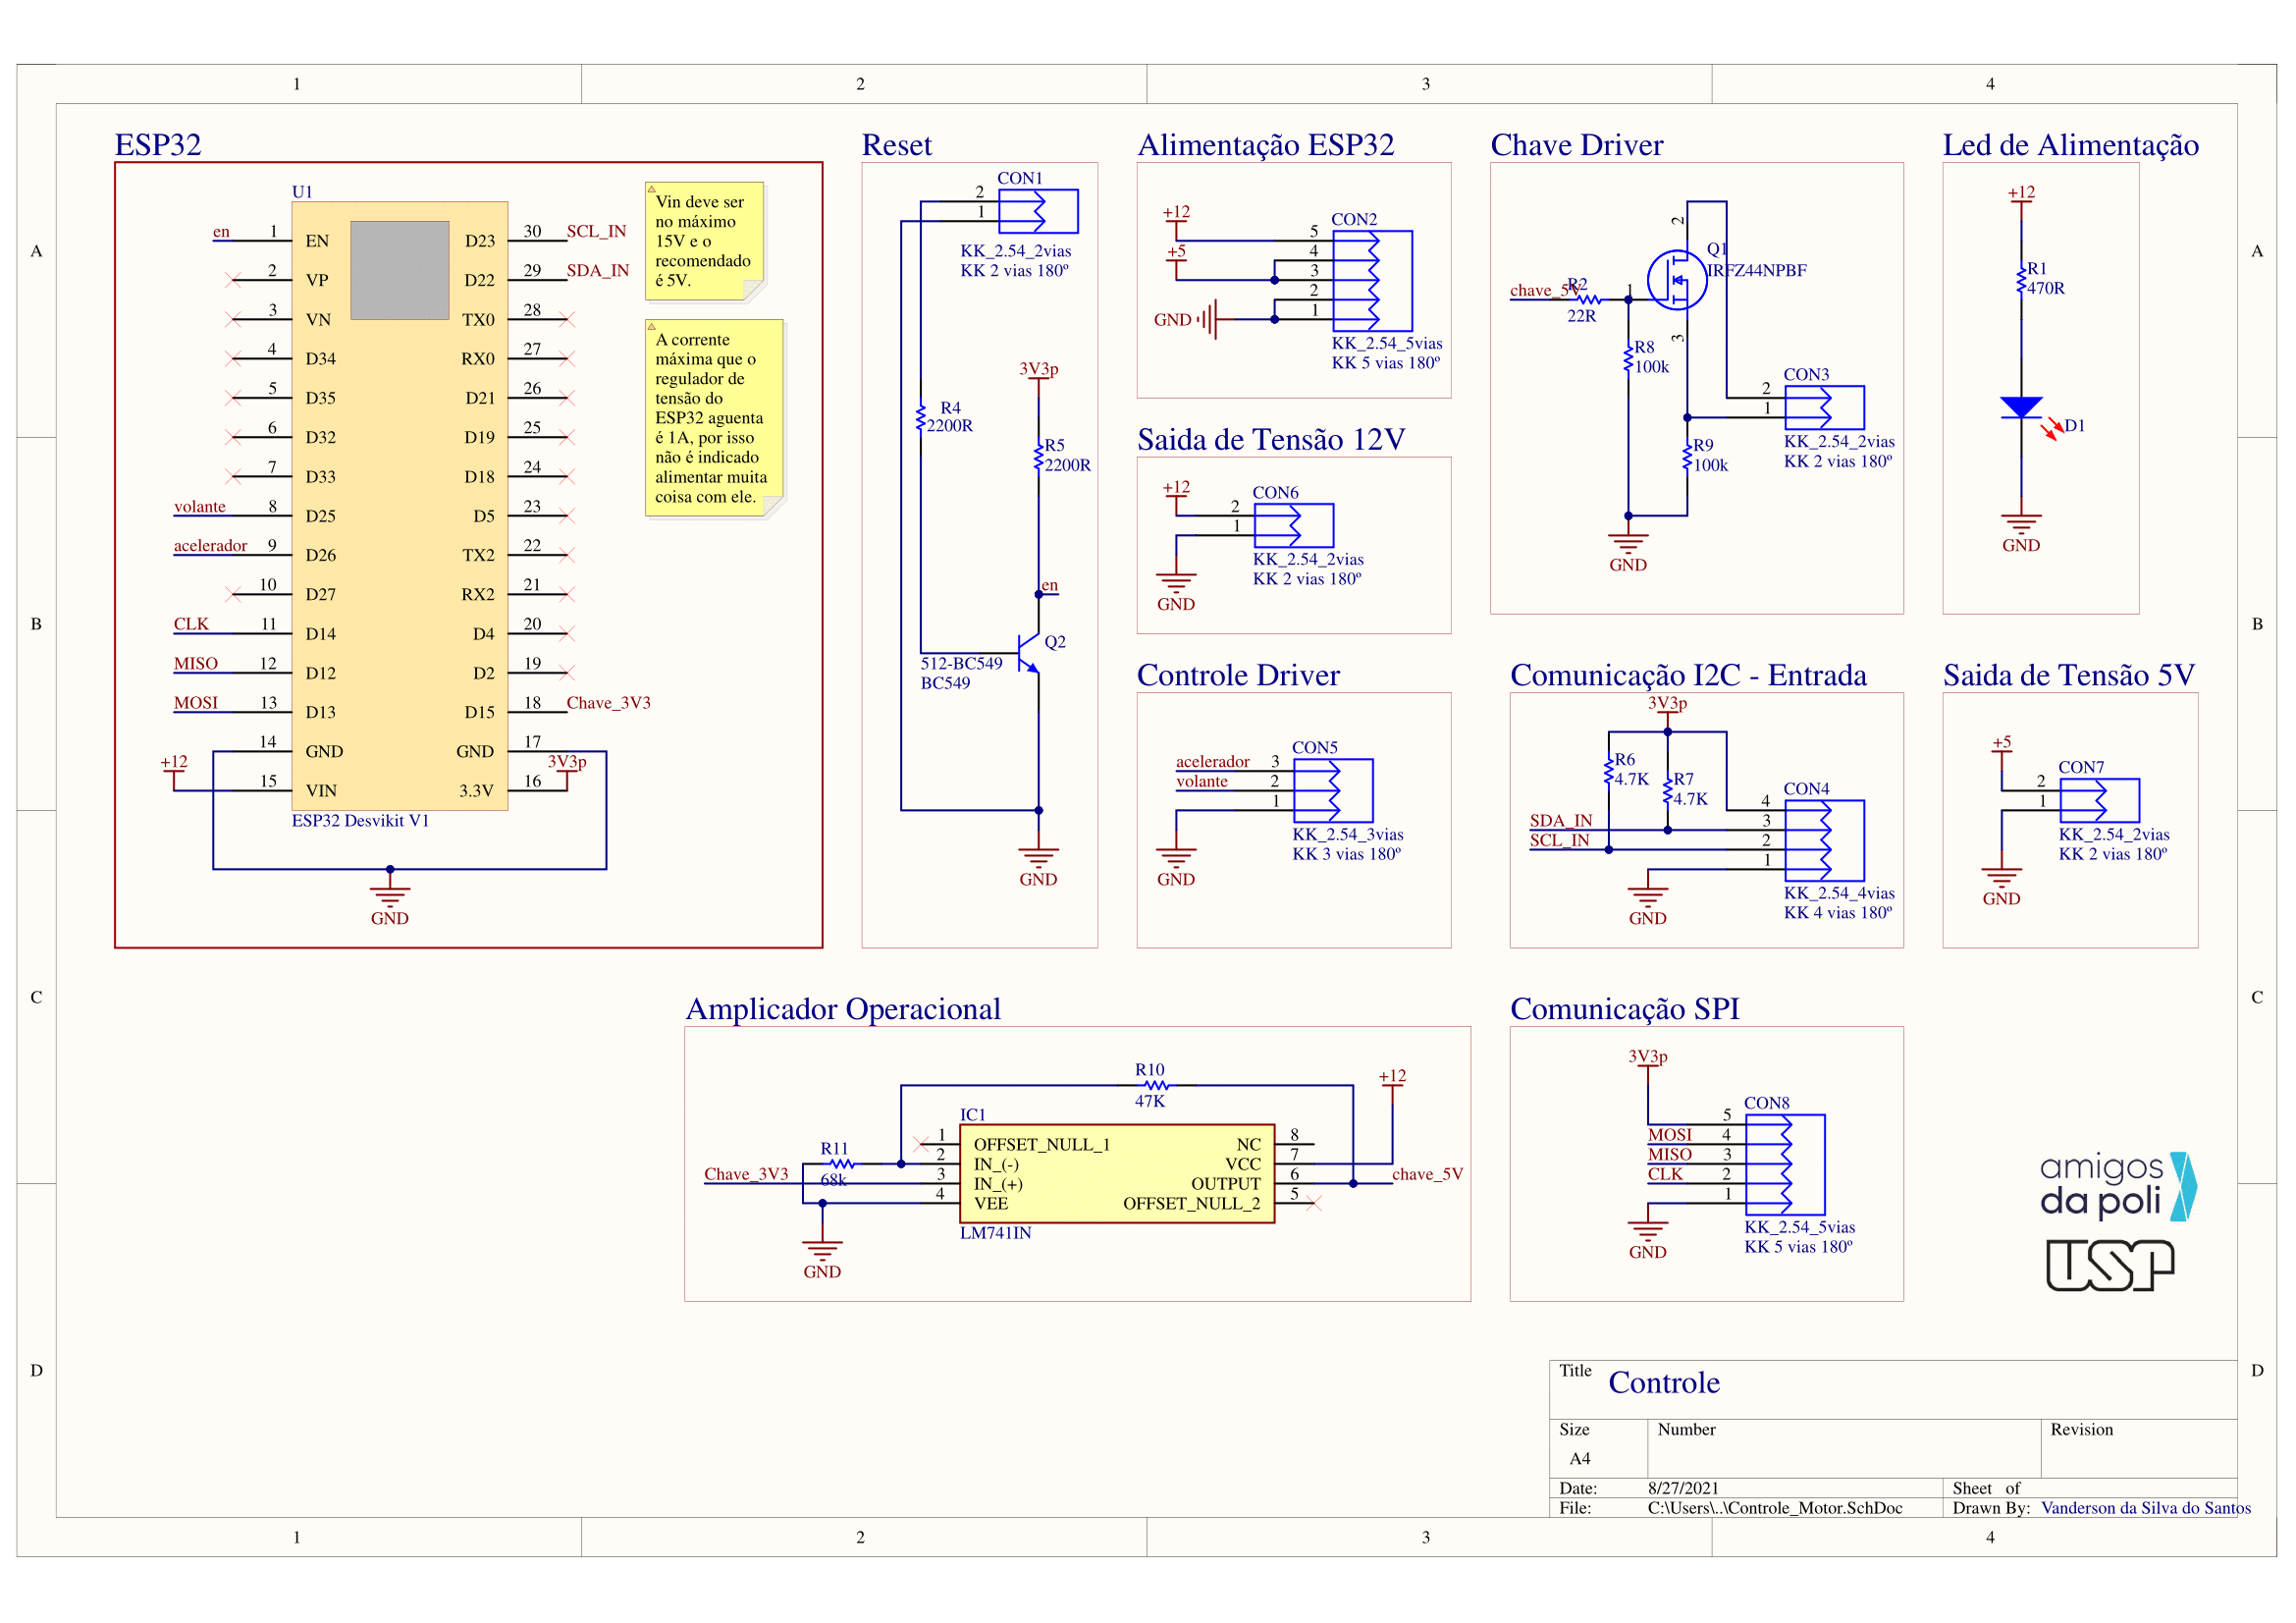
\includegraphics[width=17cm]{modulos/Controle_Motor-1.png}
    \caption*{Fonte: Elaborado pelo autor no software Altium Design\cite{altium21} }
    \label{Protótipo placa de ## - Esquemático principal}
\end{figure}

\blindtext

\begin{table}[]
\caption{Componentes Utilizados na placa de Controle - Protótipo}
\centering
\begin{adjustbox}{width=\columnwidth,center}
\begin{tabular}{|c|c|c|c|c|}
\hline
Component                   & Description                                  & Designator             & Footprint                 & Quantity \\ \hline
4.7K                      & RES 4.7K OHM 1/4W 5\% CARBON FILM            & R6, R7                 & RES 4.7K 1/4W CARBON FILM & 2        \\ \hline
47K                       & RES 4.7K OHM 1/4W 5\% CARBON FILM            & R10                    & RES 4.7K 1/4W CARBON FILM & 1        \\ \hline
68k                       & RES 4.7K OHM 1/4W 5\% CARBON FILM            & R11                    & RES 4.7K 1/4W CARBON FILM & 1        \\ \hline
BC549                     & TRANS NPN 30V 0.1A TO-92                     & Q2                     & TO92                      & 1        \\ \hline
IRFZ44NPBF                & MOSFET (N-Channel)                           & Q1                     & TO254P483X1016X1994-3P    & 1        \\ \hline
KK\_2.54\_2vias           & Conector KK 2.54mm 2 vias                    & CON1, CON3, CON6, CON7 & KK\_2VIAS\_180º           & 4        \\ \hline
KK\_2.54\_3vias           & Conector KK 2.54mm 3 vias                    & CON5                   & KK\_3vias\_180º           & 1        \\ \hline
KK\_2.54\_4vias           & Conector KK 2.54mm 4 vias                    & CON4                   & KK\_4vias\_180°           & 1        \\ \hline
KK\_2.54\_5vias           & Conector KK 2.54mm 5 vias                    & CON2, CON8             & KK\_5vias\_180°           & 2        \\ \hline
LED 5MM RED               & LED 5MM RED                                  & D1                     & LED 5MM RED               & 1        \\ \hline
LM741IN                   & Integrated Circuit                           & IC1                    & DIP762W56P254L920H508Q8N  & 1        \\ \hline
microcontrolador          & microcontrolador com moculo bluethoth e wifi & U1                     & ESP32\_Desvikit\_v1       & 1        \\ \hline
RES 470R 1/4W CARBON FILM & RES 470R OHM 1/4W 5\% CARBON FILM            & R1, R2, R4, R5, R8, R9 & RES 470R 1/4W CARBON FILM & 6        \\ \hline
\end{tabular}
\end{adjustbox}
\centering
\caption*{Fonte: Elaborado pelo autor}
\label{table:voc}
\end{table}


\paragraph{Printed Circuit board (PCB)}

\begin{figure}[!ht]
    \centering
    \begin{minipage}{0.5\textwidth}
        \centering
        \caption{Protótipo Controle - PCB 2D}
        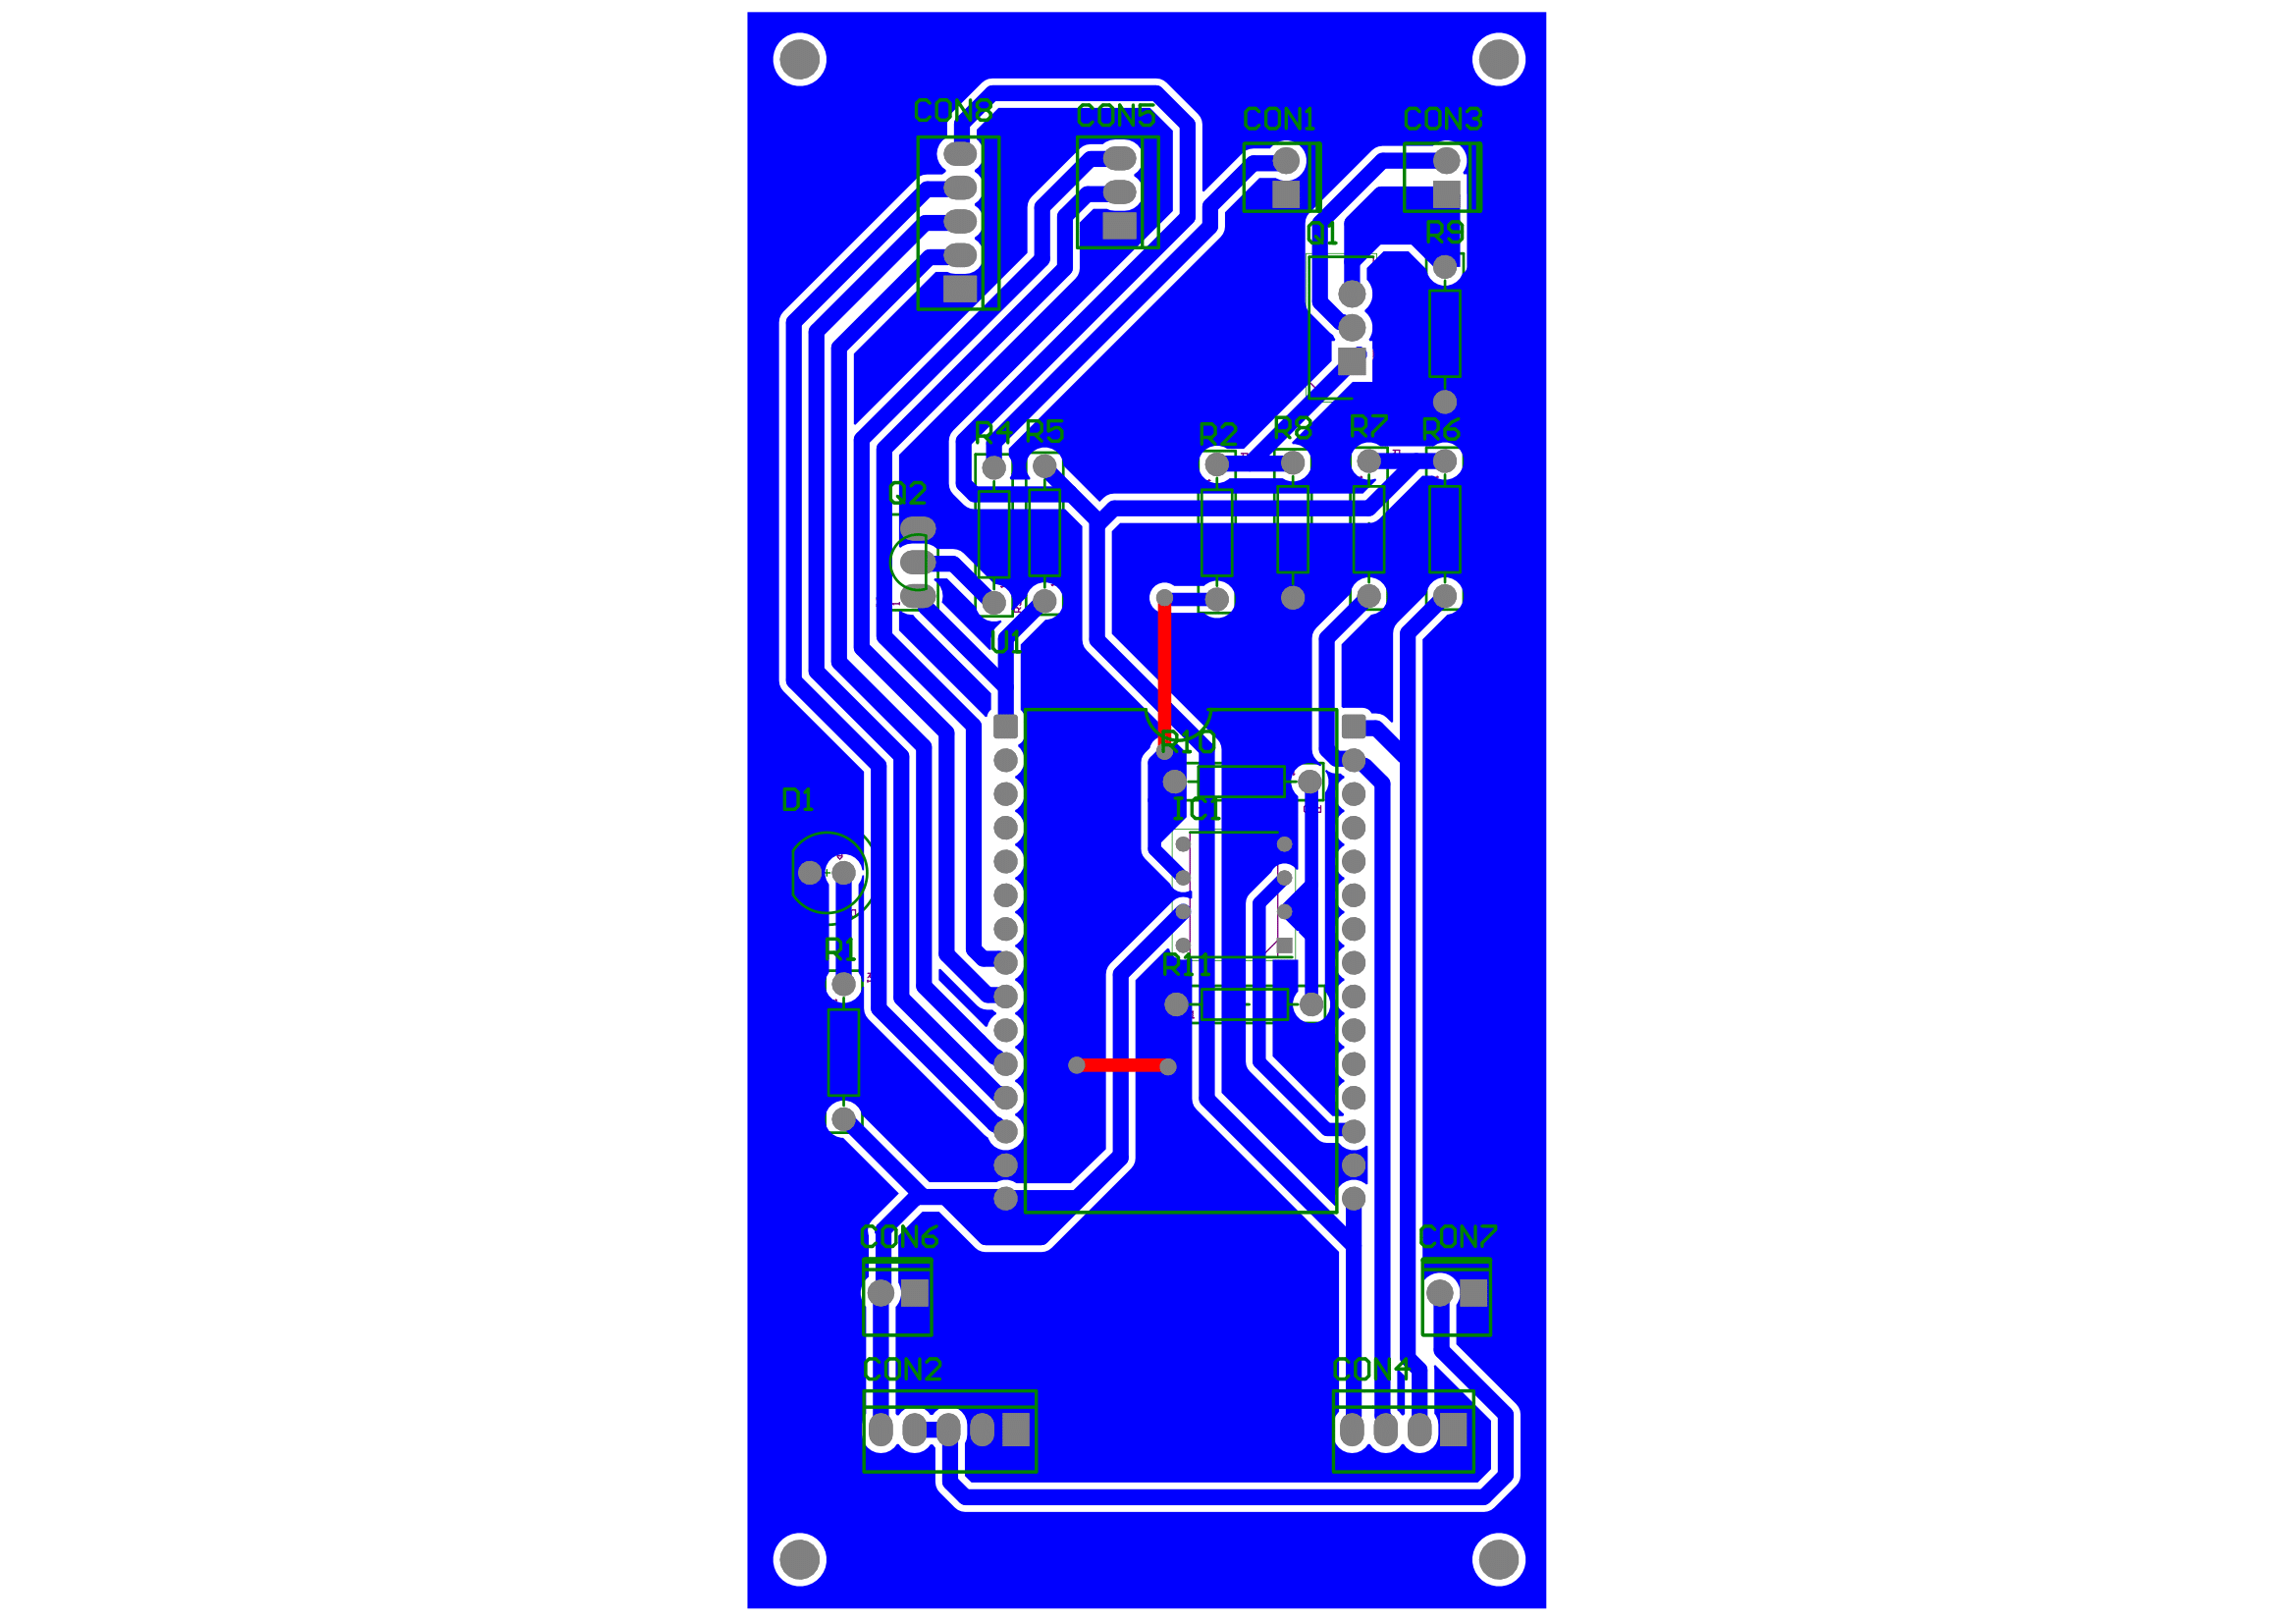
\includegraphics[width=1.03\textwidth]{modulos/Controle_Motor-2.png} 
        \label{fig:figura1minipg}
    \end{minipage}\hfill
    \begin{minipage}{0.5\textwidth}
        \centering
        \caption{Protótipo Controle - PCB 3D }
        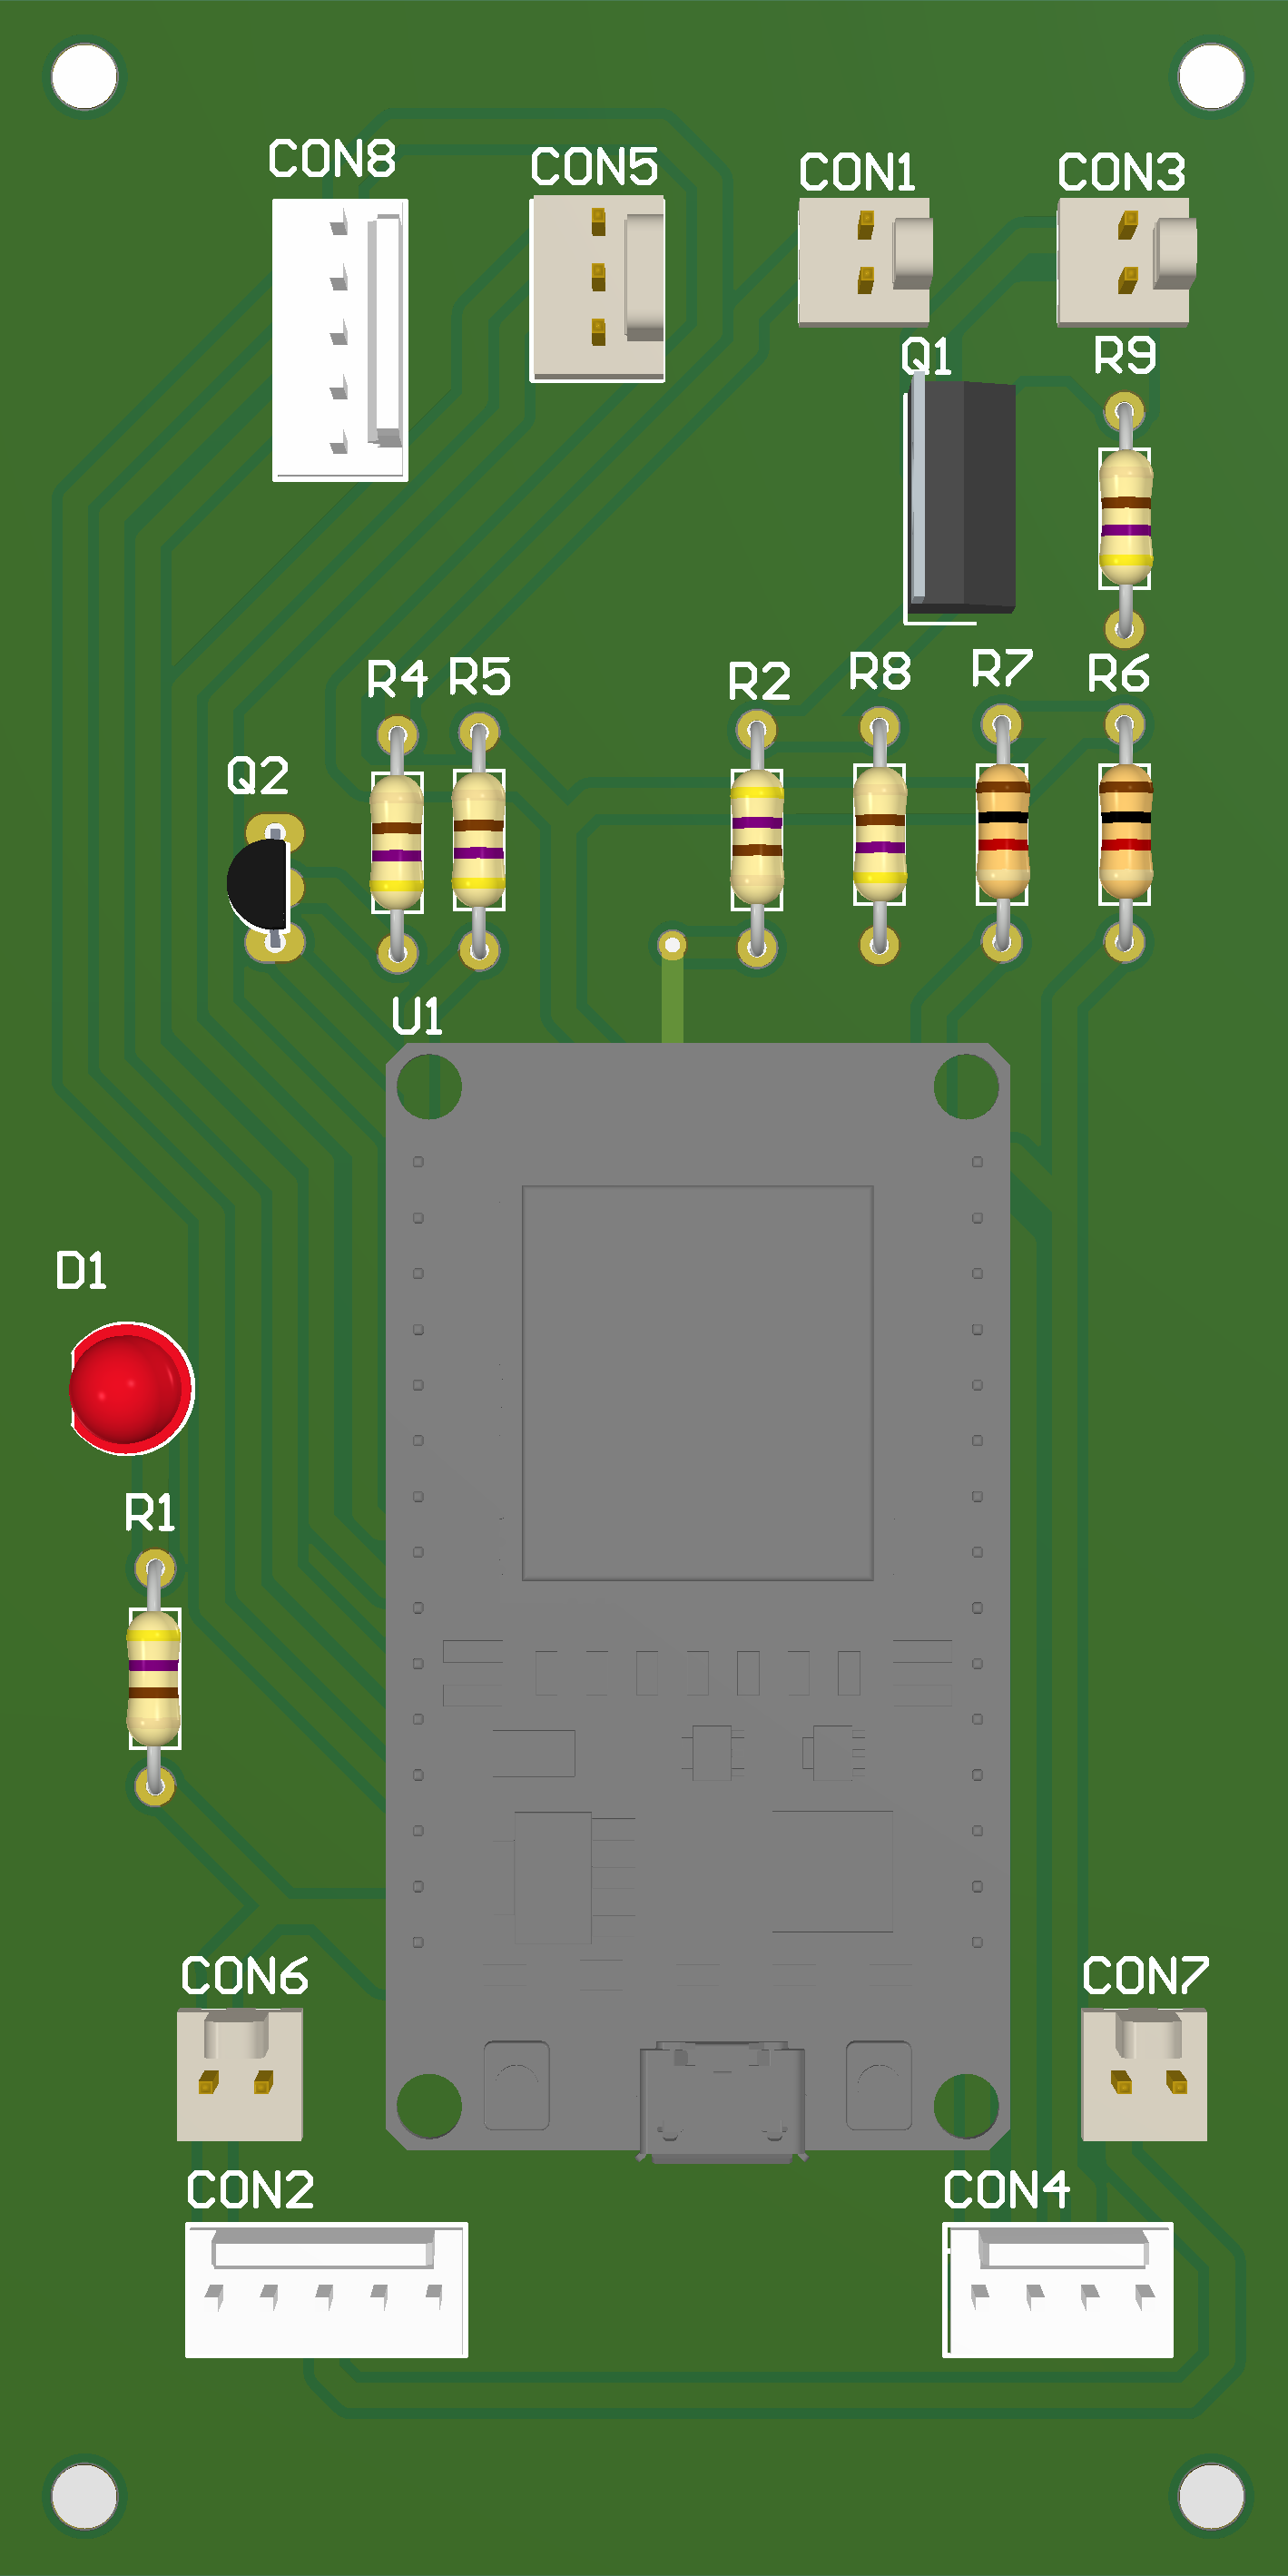
\includegraphics[width=0.4\textwidth]{modulos/Controle_Motor.png} 
        \label{fig:figura1minipg}
    \end{minipage}\hfill
    
    \caption*{Fonte: Elaborado pelo autor no software Altium Design\cite{altium21} }
    \label{fig:figurasminipg}
\end{figure}

\begin{figure}[!ht]
    \centering
    \begin{minipage}{0.5\textwidth}
        \centering
        \caption{Protótipo Controle - Trilhas}
        \includegraphics[width=0.8\textwidth]{example-image-a} 
        \label{fig:figura1minipg}
    \end{minipage}\hfill
    \begin{minipage}{0.5\textwidth}
        \centering
        \caption{Protótipo Controle - Completa }
        \includegraphics[width=0.8\textwidth]{example-image-a} 
        \label{fig:figura1minipg}
    \end{minipage}\hfill
    
    \caption*{Fonte: Elaborado pelo autor }
    \label{fig:figurasminipg}
\end{figure}

%================================ CONTROLE OFICIAL ========================
\subsubsection{Oficial}

\paragraph{Esquemático}

\begin{figure}[h]
\centering
    \caption{placa de Controle - Esquemático principal }
    \centering % para centralizarmos a figura
    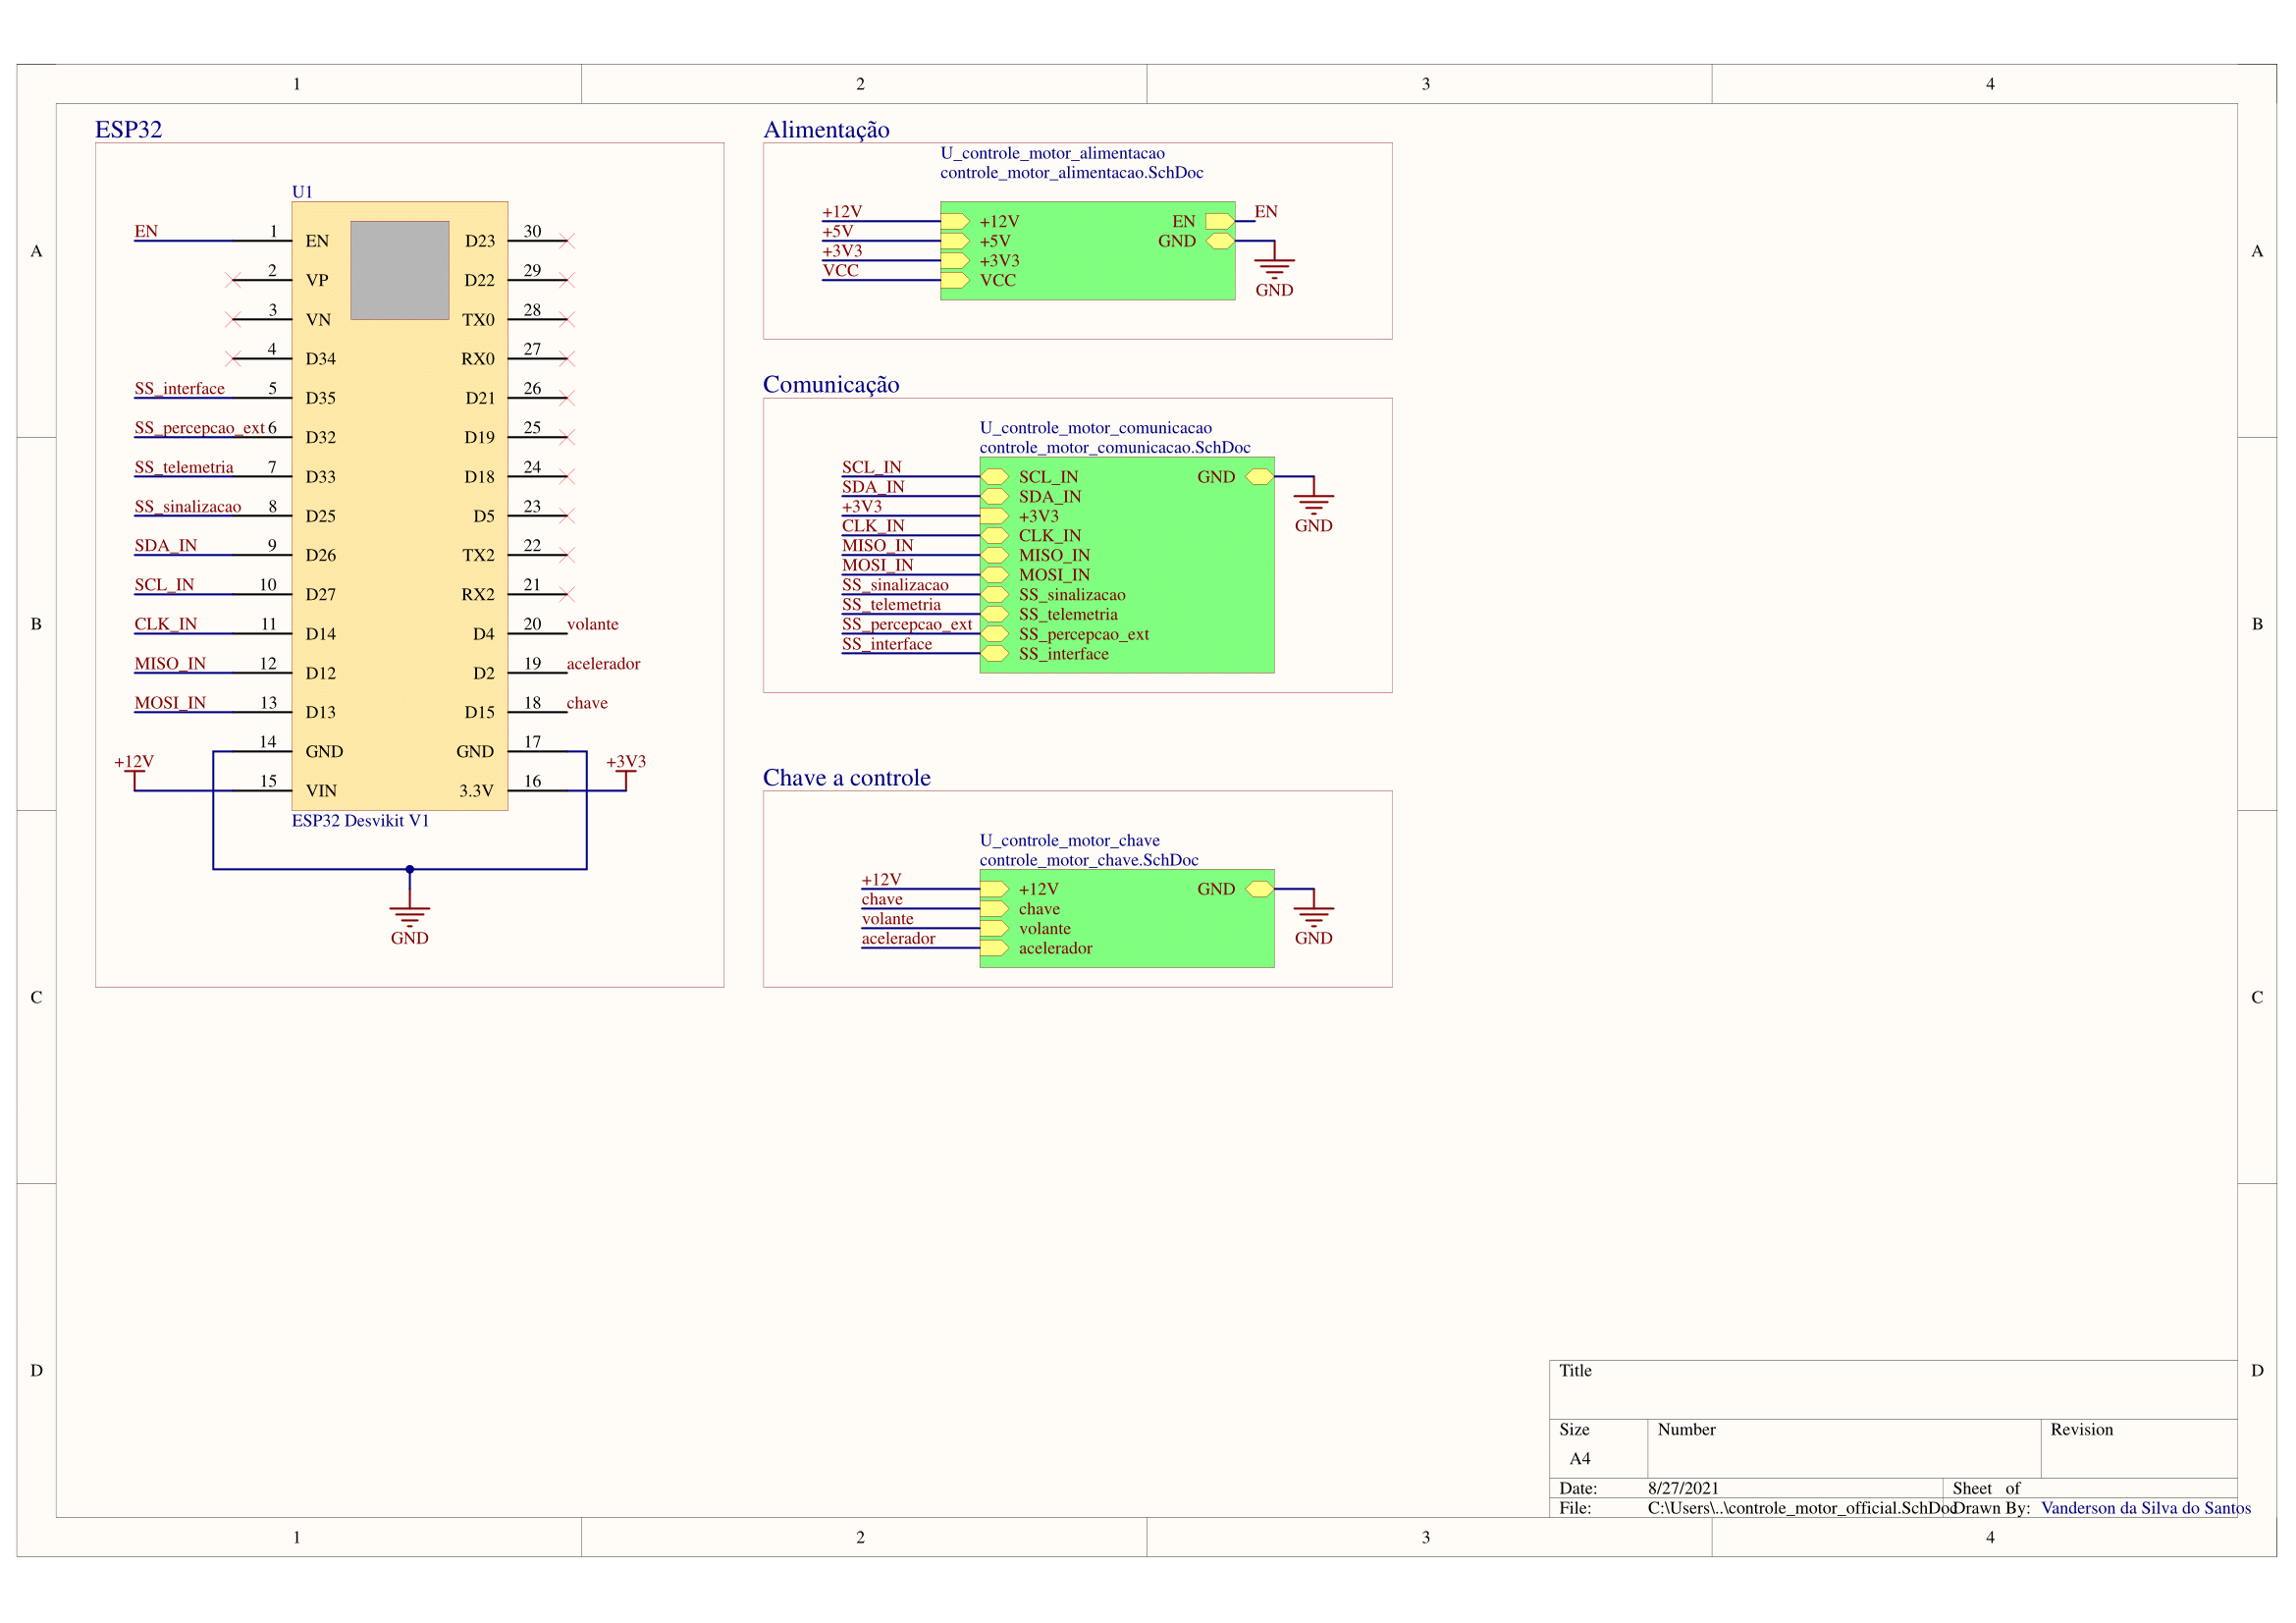
\includegraphics[width=17cm]{modulos/controle_motor_official-1.png}
    \caption*{Fonte: Elaborado pelo autor no software Altium Design\cite{altium21} }
    \label{Protótipo placa de ## - Esquemático principal}
\end{figure}

\begin{table}[]
\caption{Componentes Utilizados na placa de Controle}
\centering
\begin{adjustbox}{width=\columnwidth,center}
\begin{tabular}{|c|c|c|c|c|}
\hline
Component        & Description                                    & Designator                 & Footprint                & Quantity \\ \hline
KK\_2.54\_5vias  & Conector KK 2.54mm 5   vias                    & CON1, CON7, CON10,   CON11 & KK\_5vias\_180°          & 4        \\ \hline
KK\_2.54\_4vias  & Conector KK 2.54mm 4   vias                    & CON2                       & KK\_4vias\_180°          & 1        \\ \hline
KK\_2.54\_2vias  & Conector KK 2.54mm 2   vias                    & CON3, CON5, CON6,   CON8   & KK\_2VIAS\_180º          & 4        \\ \hline
KK\_2.54\_6vias  & Conector KK 2.54mm 6   vias                    & CON4                       & KK\_6vias\_180°          & 1        \\ \hline
KK\_2.54\_3vias  & Conector KK 2.54mm 3   vias                    & CON9                       & KK\_3vias\_180º          & 1        \\ \hline
LED 3MM RED      & LED 3MM RED                                    & D1                         & LED RED                  & 1        \\ \hline
LM741IN          & Integrated Circuit                             & IC1                        & DIP762W50P254L712H450Q6N & 1        \\ \hline
Trans BC817      & Transistor BJT NPN   BC817-25-7-F              & Q1                         & SOT96P240X110-3N         & 1        \\ \hline
IRFZ44NPBF       & MOSFET (N-Channel)                             & Q2                         & TO254P483X1016X1994-3P   & 1        \\ \hline
4k7              & RES 1206 5\%                                   & R1, R2                     & RESC3216X60N             & 2        \\ \hline
680R             & Resistor                                       & R3                         & RESC3216X60N             & 1        \\ \hline
2k2              & Resistor                                       & R4, R5                     & RESC3216X60N             & 2        \\ \hline
47K              & RES 1206 5\%                                   & R6                         & RESC3216X60N             & 1        \\ \hline
68k              & 0805                                           & R7                         & RESISTOR 0805            & 1        \\ \hline
22R              & RES 1206 5\%                                   & R8                         & RESC3216X60N             & 1        \\ \hline
100k             & RES 1206 5\%                                   & R9, R10                    & RESC3216X60N             & 2        \\ \hline
microcontrolador & microcontrolador com   moculo bluethoth e wifi & U1                         & ESP32\_Desvikit\_v1      & 1        \\ \hline

\end{tabular}
\end{adjustbox}
\centering
\caption*{Fonte: Elaborado pelo autor}
\label{table:voc}
\end{table}

%================================ CONTROLE FIRMWARE ========================
\subsection{Firmware}

\end{document}